\chapter{Psalm 21}

\begin{figure}
  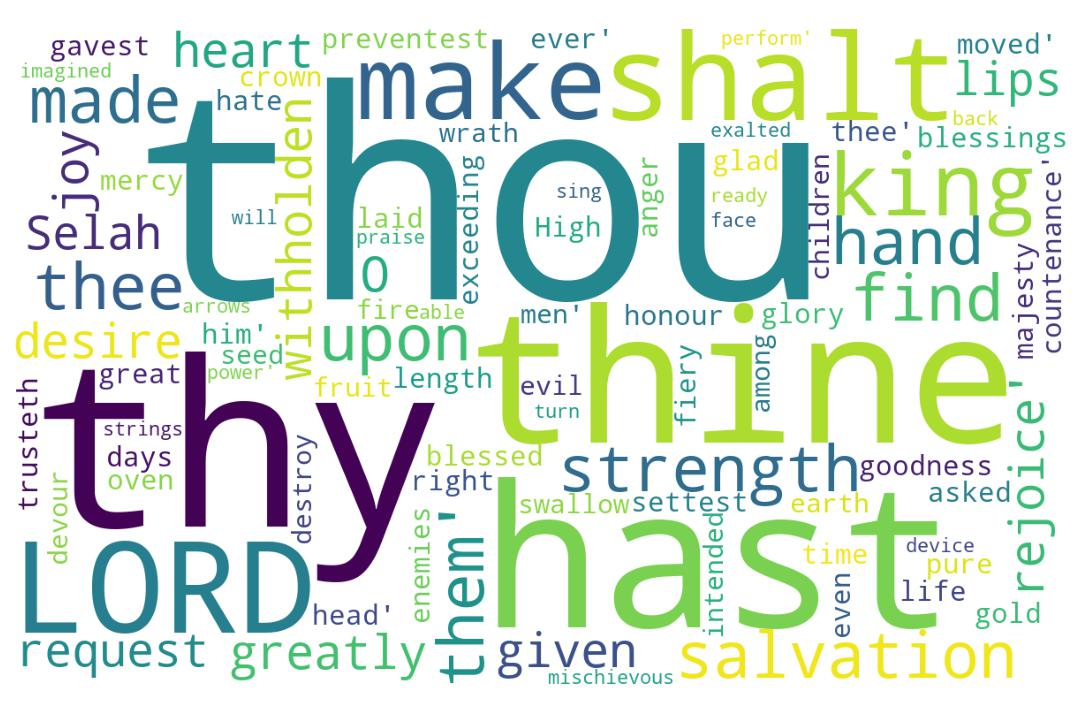
\includegraphics[width=\linewidth]{19OT-Psalms/Psalm21-WordCloud.jpg}
  \caption{Psalm 21 Word Cloud}
  \label{fig:Psalm 21 word Cloud}
\end{figure}

\marginpar{\scriptsize \centering \fcolorbox{bone}{lime}{\textbf{A GLIMPSE OF THE KING}}\\ (Psalm 21:1--13) \begin{compactenum}[I.][8]
    \item He has \textbf{Eternal Life} \index[scripture]{Psalms!Psa 021:04}(Psa 21:4)
    \item He has \textbf{Exceeding Glory} \index[scripture]{Psalms!Psa 021:05}(Psa 21:5)
    \item He has \textbf{Endless Majesty \& Honor} \index[scripture]{Psalms!Psa 021:05}(Psa 21:5)
    \item He has \textbf{Everlasting Blessing} \index[scripture]{Psalms!Psa 021:06}(Psa 21:6)
    \item He has \textbf{Enemies Destroyed} \index[scripture]{Psalms!Psa 021:08-10}(Psa 21:8-10)
    \item He has \textbf{Enormous Power} \index[scripture]{Psalms!Psa 021:13}(Psa 21:13)
\end{compactenum}}

\footnote{\textcolor[cmyk]{0.99998,1,0,0}{\hyperlink{TOC}{Return to end of Table of Contents.}}}\footnote{\href{https://www.audioverse.org/english/audiobibles/books/ENGKJV/O/Ps/1}{\textcolor[cmyk]{0.99998,1,0,0}{Psalms Audio}}}\textcolor[cmyk]{0.99998,1,0,0}{To the chief Musician, A Psalm of David.}\\
\\
\textcolor[cmyk]{0.99998,1,0,0}{The king shall joy in thy strength, O LORD; and in thy salvation how greatly shall he rejoice!}
[2] \textcolor[cmyk]{0.99998,1,0,0}{Thou hast given him his heart's desire, and hast not withholden the request of his lips. Selah.}\footnote{\textbf{Psalm 10:3} - For the wicked boasteth of his heart’s desire, and blesseth the covetous, whom the LORD abhorreth.}\footnote{\textbf{Romans 10:1} - Brethren, my heart’s desire and prayer to God for Israel is, that they might be saved.}
[3] \textcolor[cmyk]{0.99998,1,0,0}{For thou preventest him with the blessings of goodness: thou settest a crown of pure gold on his head.}
[4] \textcolor[cmyk]{0.99998,1,0,0}{He asked life of thee, \emph{and} thou gavest \emph{it} him, \emph{even} length of days \fcolorbox{bone}{lime}{for ever and ever}.}
[5] \textcolor[cmyk]{0.99998,1,0,0}{His \fcolorbox{bone}{lime}{glory} \emph{is} great in thy salvation: \fcolorbox{bone}{lime}{honour and} \fcolorbox{bone}{lime}{majesty} hast thou laid upon him.}
[6] \textcolor[cmyk]{0.99998,1,0,0}{For thou hast made him \fcolorbox{bone}{lime}{most blessed} for ever: thou hast made him exceeding glad with thy countenance.}
[7] \textcolor[cmyk]{0.99998,1,0,0}{For the king trusteth in the LORD, and through the mercy of the most High he shall not be moved.}
[8] \textcolor[cmyk]{0.99998,1,0,0}{Thine hand shall find out all thine \fcolorbox{bone}{lime}{enemies}: thy right hand shall find out those that hate thee.}
[9] \textcolor[cmyk]{0.99998,1,0,0}{Thou shalt make them as a fiery oven in the time of thine anger: the LORD shall swallow them up in his wrath, and the fire shall devour them.}
[10] \textcolor[cmyk]{0.99998,1,0,0}{Their fruit shalt thou destroy from the earth, and their seed from among the children of men.}
[11] \textcolor[cmyk]{0.99998,1,0,0}{For they intended evil against thee: they imagined a mischievous device, \emph{which} they are not able \emph{to} \emph{perform}.}\footnote{\textbf{Acts 13:10} - And said, O full of all subtilty and all mischief, thou child of the devil, thou enemy of all righteousness, wilt thou not cease to pervert the right ways of the Lord?}
[12] \textcolor[cmyk]{0.99998,1,0,0}{Therefore shalt thou make them turn their back, \emph{when} thou shalt make ready \emph{thine} \emph{arrows} upon thy strings against the face of them.}
[13] \textcolor[cmyk]{0.99998,1,0,0}{Be thou exalted, LORD, in \fcolorbox{bone}{lime}{thine own strength}: \emph{so} will we sing and praise thy power.}


